
%!TEX TS-program = lualatex
%!TEX encoding = UTF-8 Unicode

%\frame[plain]{ % When including a large figure or table, you don't want to have the bottom and the top of the slides.
%\frame[shrink]{ % If you want to include lots of text on a slide, use the shrink option.


\begin{frame}
    \frametitle{Evaluation: Performance Relative to Linux Loopback Mounting}
    \vspace*{-1pt}
    \makebox[\linewidth]{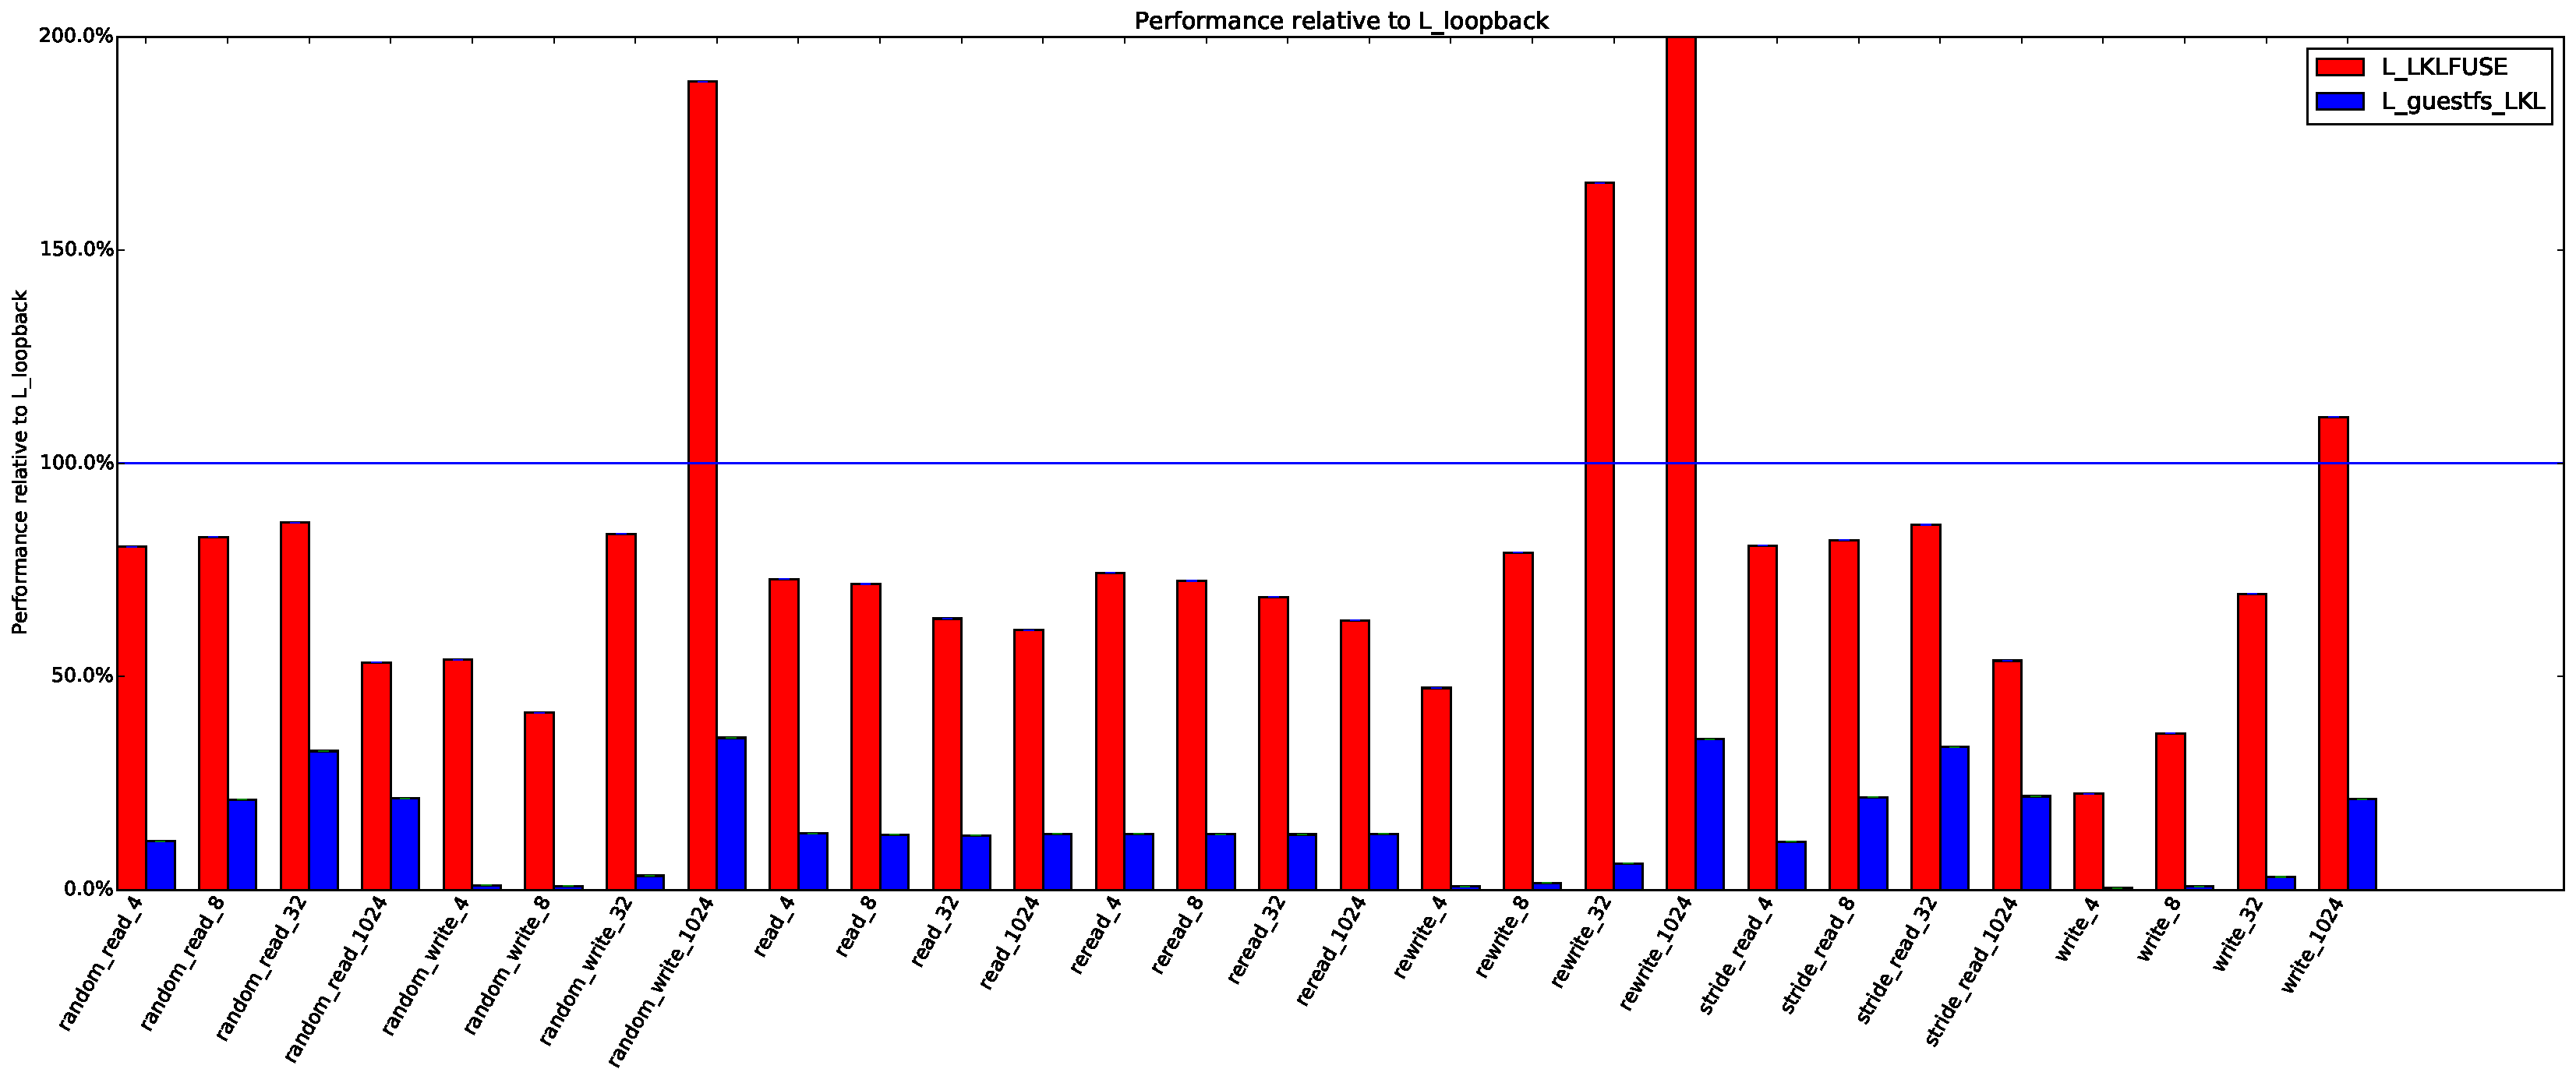
\includegraphics[page=1,width=\paperwidth]{frames/img/relative_performance_L_LKLFUSE_L_guestfs_LKL}}
    \note{
        \begin{itemize}
            \item relative, not absolute. not looking at absolute numbers
            \item not suitable for analysis, only look at individual data points
            \item provides a general picture for comparison
            \item created detailed graphs suitable for analysis of behaviour
            \item LKL delivers okay performance, i.e. above 50\%
            \item spikes are either caused by dirty-pages that got repeatedly written to without being flushed to disk or non-working sync. Need to have a closer look on mmap behaviour.
            \item many moving parts, two kernels, several caches, readahead...
            \item libguestfs-lkl is too slow
        \end{itemize}
    }
\end{frame}

\begin{frame}
    \frametitle{Evaluation: Performance Relative to Linux Loopback Mounting}
    \vspace*{-1pt}
    \makebox[\linewidth]{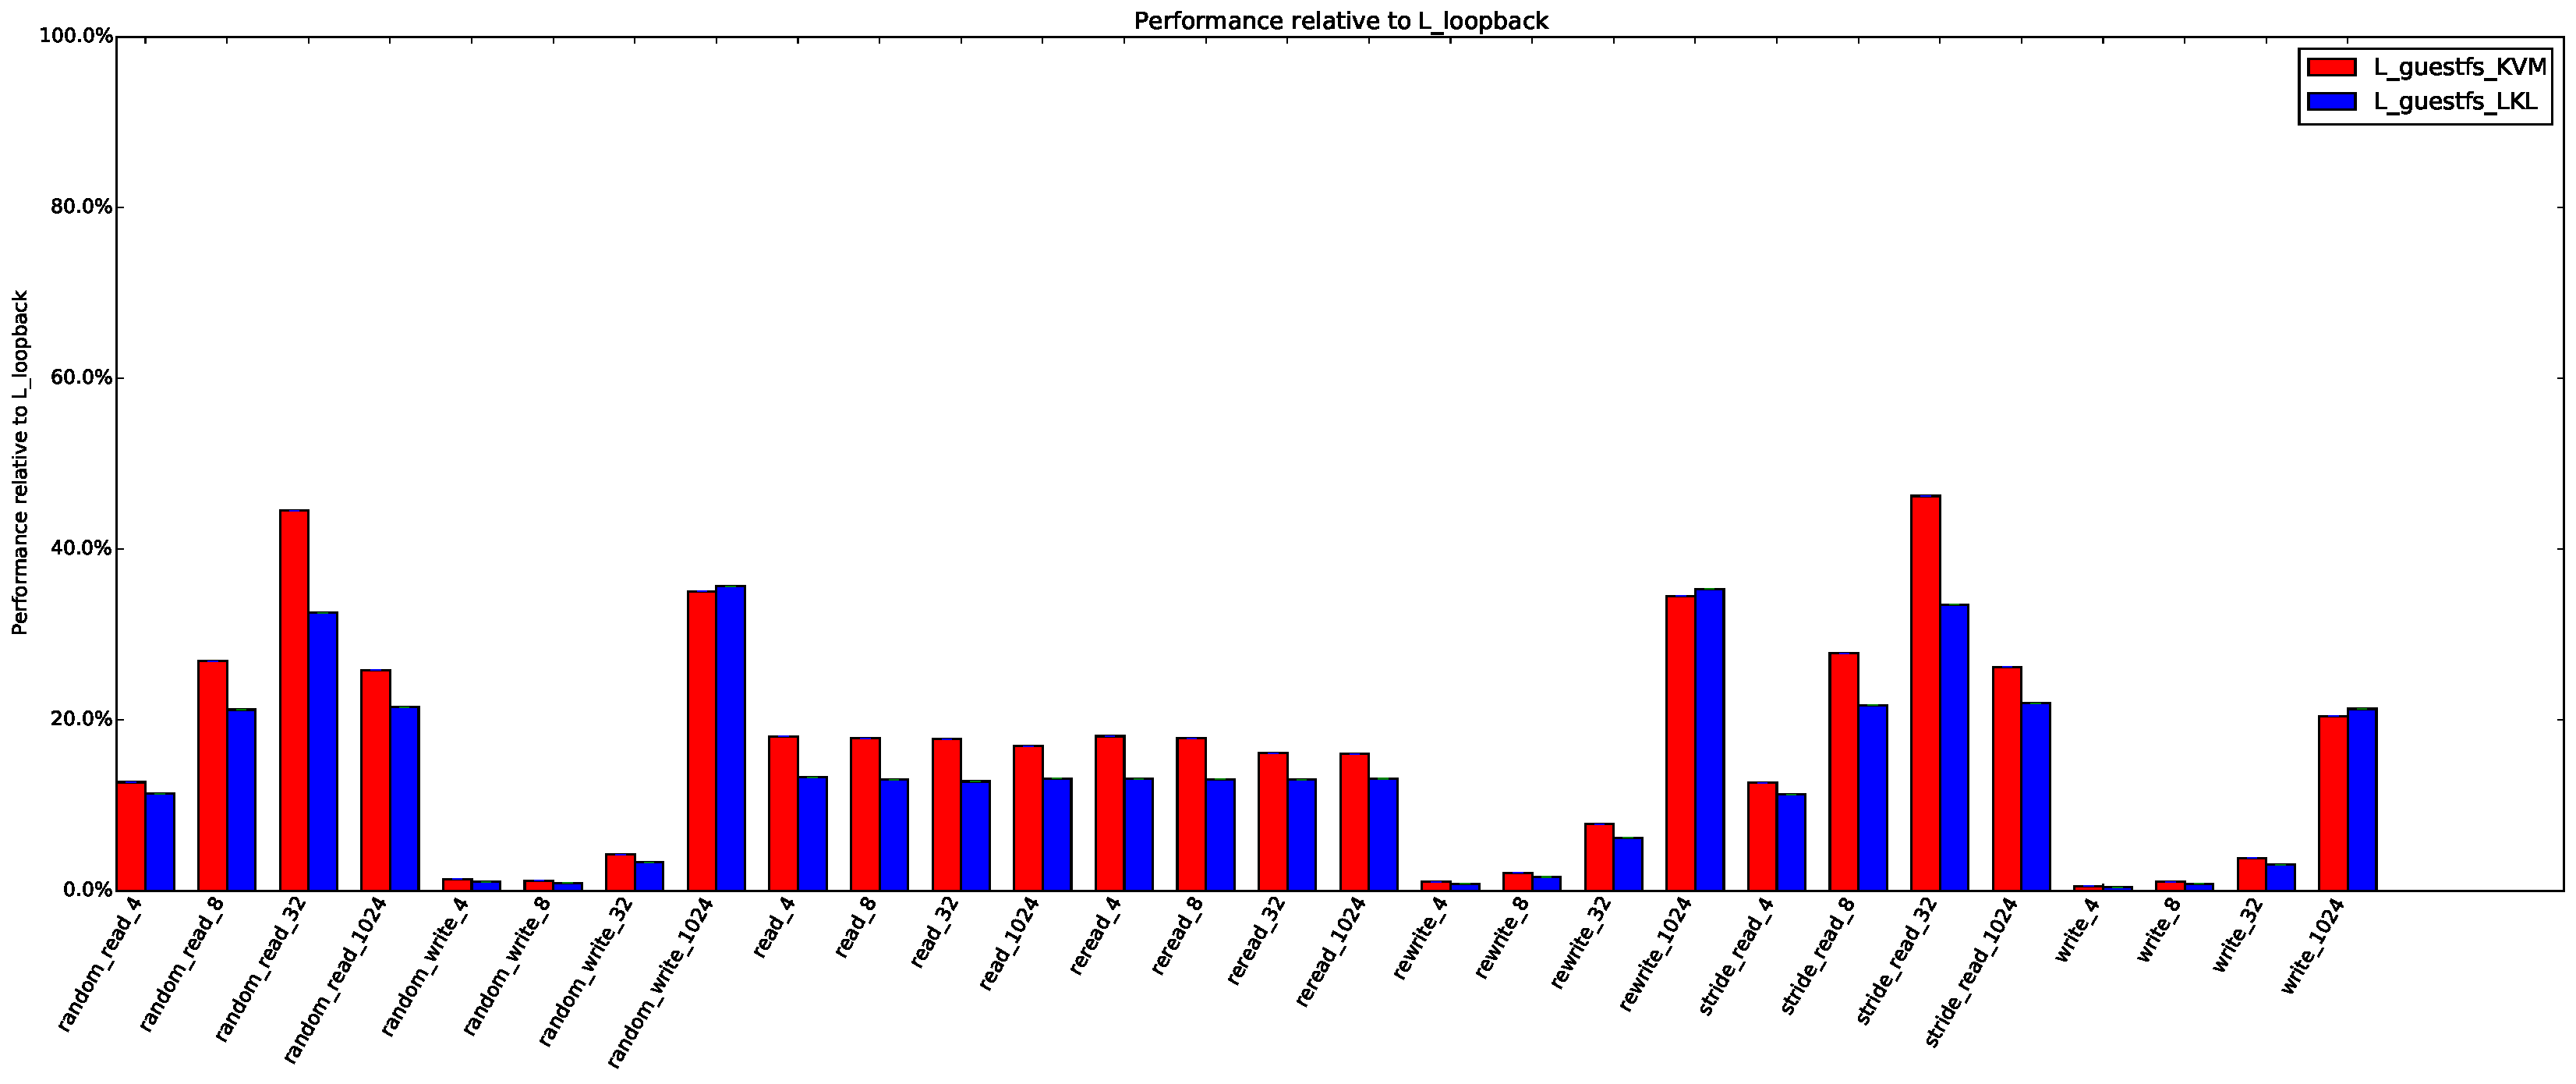
\includegraphics[page=1,width=\paperwidth]{frames/img/relative_performance_L_guestfs_KVM_L_guestfs_LKL}}
    \note{
        \begin{itemize}
            \item mostly caused by the communication protocol overhead.
            \item libguestfs-kvm is only slightly faster
            \item I expect it to be possible to optimize the prototypic LKL-backend so that it outperforms the LKL-backend
        \end{itemize}
    }
\end{frame}

\begin{frame}
    \frametitle{Evaluation: Performance Relative to Windows VHD Mounting}
    \vspace*{-1pt}
    \makebox[\linewidth]{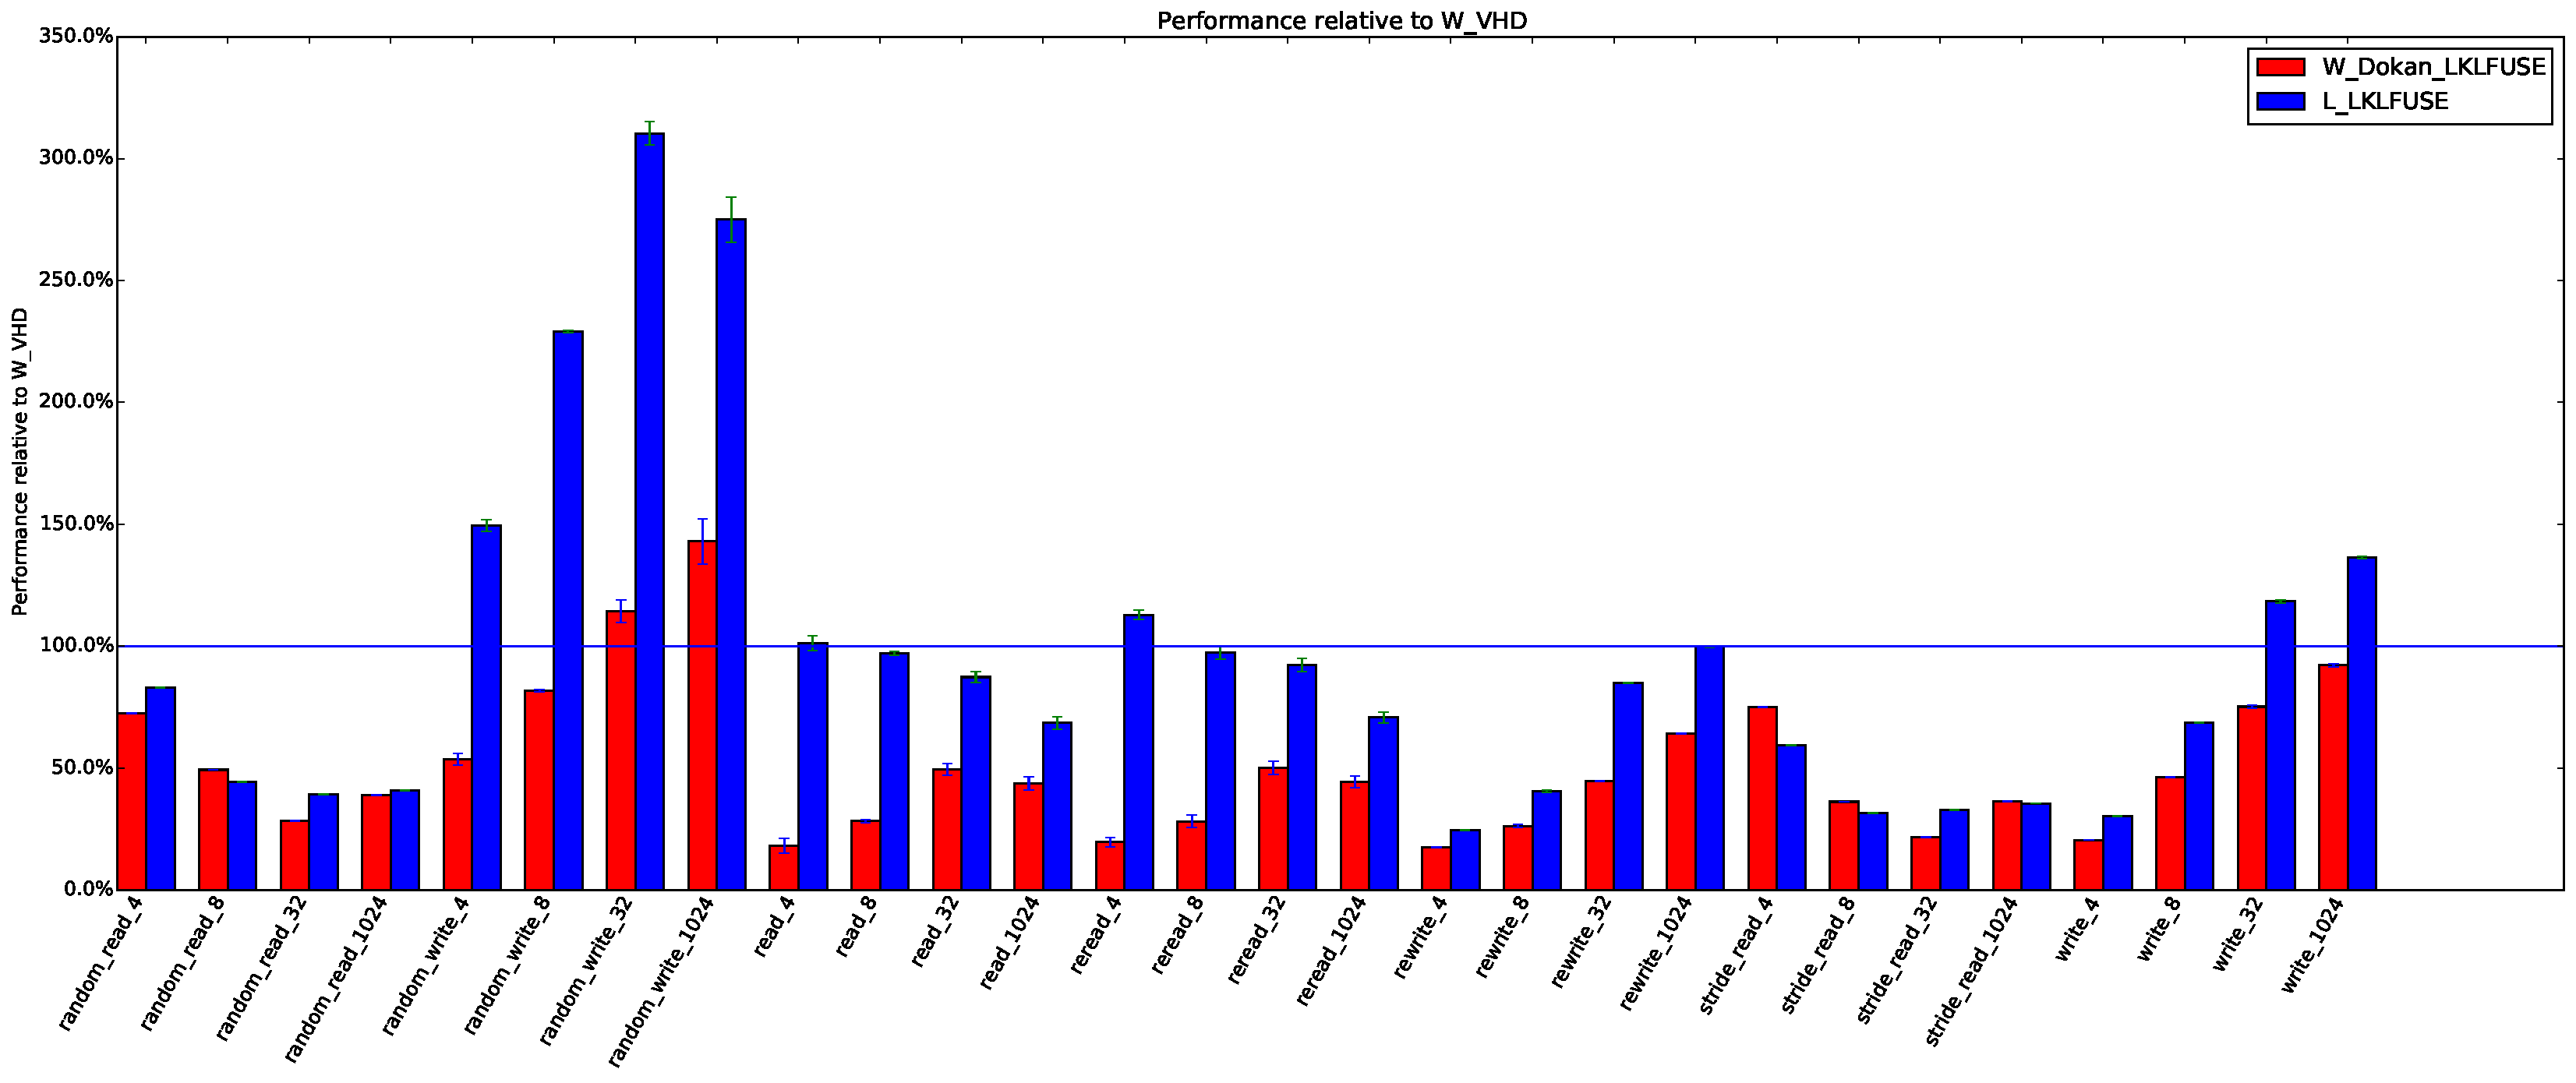
\includegraphics[page=1,width=\paperwidth]{frames/img/relative_performance_W_Dokan_LKLFUSE_L_LKLFUSE}}
    \note{
        \begin{itemize}
            \item one can see how LKLFUSE does worse under Windows than under Linux. Again, we might be comparing apples and oranges here...
            \item Dokan has several problems (no caching, fixed number of worker threads)
        \end{itemize}
    }
\end{frame}